\chapter{研究综述}

\section{即席视频检索}

本文回顾了 2016 年至 2019 年四年的 TRECVID 评测中的即席视频检索系统(Ad-hoc Video Search,AVS)~\cite{awad2016trecvid,awad2017trecvid,awad2018trecvid,awad2019trecvid}任务的效果较好的算法,因为 TRECVID 评测是最有挑战的基准,吸引了该领域包括卡耐基梅隆大学、弗吉尼亚大学、香港中文大学等学术界和阿里巴巴等工业界的一些优秀学者参与评测并且提出了很多有效的算法~\cite{}。该评测的测试数据的正确答案在参与者提交评测结果前是不公开的,并且参与者不允许为任何的查询样例调整他们的结果,这样可以公平地评价参与者的模型的泛化能力。
表格\ref{tab:method-diffs}从三个关键组成部分分析这些算法的异同,即自然语言查询是如何表示的(查询表示)、未标注的视频是如何表示的(视频表示)、在什么特征空间进行跨模态匹配(公共空间)。


\begin{table} [tbp!]
    %\renewcommand{\arraystretch}{0.95}
    \caption[AVS系统回顾]{该表格回顾了2016年至2019 TRECVID的排名前三名的AVS系统,本文围绕着三个维度描述这些系统,即1)即席查询是如何表达的,2)未被标注的候选视频集是如何表达的,3)用于计算跨模态相似度的公共空间是如何表达的。}
    \label{tab:method-diffs}
    \centering
    \scalebox{0.73}{
        \begin{tabular}{| l | l | l | l | l |}
            %\toprule
            \hline
            \textbf{排名} & \textbf{系统} & \textbf{文本表示} & \textbf{视频表示} & \textbf{公共空间} \\
            \hline
            \multicolumn{5}{|l|}{2016:} \\ \hline
            1 & Le \etal\cite{le2016nii} & \specialcell{词袋向量(Bag-of-\\words~\cite{sivic2003video})} & \specialcell{通过预训练的卷积神经网络\\(VGG-16~\cite{simonyan2014very})提取的概念特\\征向量} & 文本特征空间 \\ \hline
            2 & Markatopoulou \etal\cite{foteini2016iti} & \specialcell{基于规则的概念选择得\\到的概念特征向量~\cite{markatopoulou2017query}} & \specialcell{通过预训练的卷积神经网络\\(AlexNet~\cite{krizhevsky2012imagenet},GoogLeNet~\cite{szegedy2015going}, \\ResNet~\cite{he2016deep}, VGGNet~\cite{sivic2003video})\\提取的概念特征向量} & \specialcell{1345 维的概念\\特征空间} \\ \hline
            3 & Liang \etal\cite{liang2016inf} & word2vec~\cite{mikolov2013distributed} & \specialcell{通过预训练的卷积神经网络\\(VGG-19~\cite{simonyan2014very}, C3D~\cite{tran2015learning})\\提取的视觉特征} & 视觉特征空间 \\ \hline
            \multicolumn{5}{|l|}{2017:} \\ \hline
            1 & Snoek \etal\cite{snoek2017university} & \specialcell{词袋向量(Bag-of-\\words)~\cite{sivic2003video}} & \specialcell{由VideoStory~\cite{habibian2014videostory}模型产生\\的词袋向量(Bag-of-words)} & \specialcell{文本特征空间} \\ \hline
            2 & Ueki \etal\cite{ueki2017waseda} & \specialcell{基于规则的概念选择得\\到的概念特征向量} & \specialcell{通过预训练的卷积神经网络\\(AlexNet~\cite{krizhevsky2012imagenet}, GoogLeNet~\cite{szegedy2015going})\\提取的概念特征向量} & \specialcell{5万维的概念\\特征空间} \\ \hline
            3 & Nguyen \etal\cite{nguyen2017vireo} & \specialcell{基于规则的概念选择得\\到的概念特征向量} & \specialcell{通过预训练的卷积神经网络\\(ResNet-50)提取的概念特征\\向量} & \specialcell{2774维的概念\\特征空间} \\ \hline
            \multicolumn{5}{|l|}{2018:} \\ \hline
            1 & Li \etal\cite{li2018renmin} & \specialcell{由W2VV++~\cite{li2019w2vv++}模型产\\生的稠密向量} &  \specialcell{通过预训练的卷积神经网络\\(ResNeXt-101~\cite{xie2017aggregated}, ResNet-\\152)提取的视觉特征} & \specialcell{视觉特征空间/\\学习的隐空间} \\ \hline
            2 & Huang \etal\cite{huang2018informedia} & \specialcell{+基于规则的概念选择\\得到的概念特征向量\\+通过注意力网络得到\\的稠密向量} & \specialcell{+通过预训练的卷积神经网\\络提取的概念特征向量\\+通过预训练的卷积神经网\\络提取的视觉特征} & \specialcell{+概念特征空间\\+学习的隐空间} \\ \hline
            3 & Bastan \etal\cite{bastan2018ntu} & \specialcell{由VSE++~\cite{faghri2017vse++}模型得到\\的稠密向量} & \specialcell{通过预训练的卷积神经网络\\(ResNet-152)提取的视觉特征} & \specialcell{学习的隐空间} \\ \hline
            \multicolumn{5}{|l|}{2019:} \\ \hline
            1 & Wu \etal\cite{wu2019hybrid} & \specialcell{混合文本编码策略} & \specialcell{混合视觉特征编码策略} & \specialcell{学习的隐空间} \\ \hline
            2 & Li \etal\cite{li2019renmin} & \specialcell{由W2VV++~\cite{li2019w2vv++}模型产\\生的稠密向量} & \specialcell{通过预训练的卷积神经网络\\(ResNeXt-101, ResNet-152)\\提取的视觉特征} & \specialcell{视觉特征空间/\\学习的隐空间} \\ \hline
            3 & Ueki \etal\cite{ueki2019waseda} & \specialcell{由VSE++~\cite{faghri2017vse++}模型得到\\的稠密向量} & \specialcell{通过预训练的卷积神经网络\\(ResNet-50, ResNet-101,\\ ResNet-152)提取的视觉特征} & \specialcell{学习的隐空间} \\ \hline
            %\bottomrule
        \end{tabular}
    }
\end{table}


在 TRECVID 2016 评测中,Le等人在文献~\cite{le2016nii}中提出一种基于文本查询的解决算法。他们先用预
训练的卷积神经网络(VGG-16)对视频中的帧图像提取语义概念特征,包括主要的物体、场景属性、
物体之间的关系等。在获取视频的语义概念后,视频查询任务就转化成了文本查询任务,即以查询的文本检索视频的概念,
他们使用标准的 TF-IDF 技术来计算每个概念特征的权重。给定的查询与视频的相似度由查询
文本与视频的概念特征在文本空间中计算得出。
Markatopoulou等人~\cite{foteini2016iti}提出了一种类似的算
法,即先通过预训练的卷积神经网络(AlexNet, GoogLeNet, ResNet 和 VGGNet)来提取视
频关键帧的 1000 维 ImageNet~\cite{russakovsky2015imagenet}的概念特征和 345 维 TRECVID SIN~\cite{smeaton2009high}的概念特征,把两
类特征做拼接并且将通过这四个深度卷积网络得到的特征取平均来表示视频, 每一个概念
的维度上的数值表示该概念在视频中出现的概率。在文本表示上,他们通过显式语义分析(ESA~\cite{gabrilovich2007computing})的方
式来计算查询文本与视频的 1345 个概念之间的相关性,如果这个相关性大于一个给定的阈值,则
选择这个概念来表示这个查询文本。不同于前两种算法,Liang 等人~\cite{liang2016inf}使用 webly-labeled
learning~\cite{liang2016learning}算法来对每个查询进行建模,即先通过word2vec的稠密向量进行表示,而视频则使用VGG-19和C3D提取视觉特征。
为了解决零样本的问题,他们利用查询文本从Youtube 上爬取了弱标注的视频数据来训练模型,尽管这种方法被证明有效果~\cite{kordumova2015best},但是对于一些复杂的查询来说,从网上自动爬取相关的视频还是很困难的。因此在实际的评测中,这种方法不如前两种方法有效。

在 TRECVID 2017 评测中,尽管基于概念的查询和特征表示仍然很主流,获得评测第
一名的 Snoek 等人在文献\cite{snoek2017university}中提出一种更加优雅的表示方式——VideoStory~\cite{habibian2014videostory}。对于每个没有标注的视频,他们利用深度卷积神经网络提取深度特征,并通过线性变换将该特征转换到
VideoStory 空间进行表示。这个表示进一步通过线性变换转换为词袋向量(Bag-of-words,bow),而每个查
询也用词袋向量进行表示。因此,视频与查询间的余弦相似度可以在词袋向量空间直接进行
计算。尽管这种方法效果很好,但是也存在两个明显的不足:第一,词袋向量(bow)
忽略了查询语句的时序信息;第二,词袋向量的有效性依赖于合适的词典选择,但这是无法
和表示学习一同进行优化的,即一旦确定了词典,则所有文本的表示都是固定的。
相反,本文提出的通过深度神经网络来表示查询既考虑了词语
的重要性,也考虑了词语间的时序信息,并且可以端到端地进行训练优化文本查询的表示。
而第二名的Ueki等人~\cite{ueki2017waseda}使用Alexnet和GoogLeNet分别在ImageNet~\cite{deng2009imagenet}、Places~\cite{zhou2014learning}、FCVID~\cite{jiang2017exploiting}、UCF101~\cite{soomro2012ucf101}等
数据集上收集了包括物体、场景、动作等一共5万维的概念向量组成了一个很大的概念库,而Nguyen等人~\cite{nguyen2017vireo}使用了类似的方案,他们使用ResNet-50提取了2774维的概念向量,评测结果排在第三名,由此可以合适的概念选择对检索的效果影响很大。

在 TRECVID 2018 评测中,许多基于深度学习的方法来表示查询的方案出现了。
Huang等人~\cite{huang2018informedia}使用了两种方法,第一种方法是基于概念的方法,即先使用预训练的深度卷积神经网络
在YFCC~\cite{thomee2016yfcc100m},ImageNet Shuffle~\cite{mettes2016the},UCF101~\cite{soomro2012ucf101},Kinetics~\cite{carreira2017quo},Places~\cite{zhou2014learning},Google Sports~\cite{karpathy2014large}等数据上提取了一共13,626维的概念向量,而文本表示则通过基于规则的概念选择得到文本的概念向量表示,最终文本查询与候选视频的相似度在概念向量空间计算得到。第二种方法是通过联合嵌入空间的方法为文本学习连续的向量表示,即先用预训练的卷积神经网络Inception-v4~\cite{szegedy2016inception}提取视频的视觉特征,然后他们叠加了两个注意力模型Dual Attention Network~\cite{nam2017dual}和Stacked Cross-Attention Network~\cite{lee2018stacked},学习一个子空间来计算跨模态的相似度。最终,他们后融合这两种方法的结果。
而Bastan等人~\cite{bastan2018ntu}使用 VSE++~\cite{faghri2017vse++}模型,即先使用预训练的ResNet-152提取视频的视觉特征,使用Gated Recurrent Unit(GRU)~\cite{cho2014learning}编码查询文本,然后为两个模态表示学习一个公共的子空间,该方法获得了评测的第三名。而本文研究的基于深度学习的方法W2VV++取得评测的第一名。

在 TRECVID 2019 评测中,排名前三的方法都是基于深度学习的。
排在第一名的Wu等人\cite{wu2019hybrid}使用了混合的序列编码策略对视频特征和文本的词向量进行聚合建模。由于查询句子和视频都是序列的模态,即视频由一系列的图像组成,句子由一系列的单词组成,因此视频深度特征通常是先对视频提取帧图像,然后再对图像使用卷积神经网络ResNet-152到的是一系列的图像特征,同样句子先经过word2vec模型得到一系列的单词的词向量。为了得到最终的视频表示和句子表示,他们使用平均池化、GRU~\cite{cho2014learning}、NetVLAD~\cite{arandjelovic2016netvlad}和图卷积网络~\cite{mao2018hierarchical}的方式对这些序列的特征进行聚合表达成视频向量和句子向量,然后通过拼接的方式相对应地融合这些特征来作视频和句子的最终向量表示,最后他们为这两个模态的向量联学习一个公共的子空间。

\section{跨模态检索的特征融合}
即席视频检索本质上是一个以文本搜视频的跨模态检索问题,因此本文也关注到一些基于深度学习解决文本-视频的跨模态匹配任务的工作。
因为文本-视频的跨模态匹配的核心是计算文本与视频的相关度,而文本与视频具有的异构性的特点,因此需要把它们投到异构公共的空间计算,而在这之前则需要分别对文本和视频进行向量化表示。
视频是由一序列的帧图像和一段音频组成,既包括了静态的对象也含有动态的对象,通常还含有音频信息,是非常复杂的多媒体数据,因此对视频进行准确地向量表示也是困难的。
Ueki等人~\cite{ueki2019waseda}为了充分提取视频的图像信息,使用了ResNet-50,ResNet-101和ResNet-152三种深度卷积神经网络提取视频的帧图像视觉特征,并且为每个特征单独地学习一个文本-视频联合的公共子空间,最后使用平均后融合的方式融合这些子空间从而得到最终的视频检索结果。虽然他们使用不同的深度卷积神经网络提取视频的特征,但这几种神经网络提取的特征是很相似的,它们的网络结构是类似的,只是网络的层数逐渐更多更深,因此提取到的特征只是表达效果越来越好,但特征间缺乏互补性。考虑到视频的音频信息和动态信息,Mithun等人~\cite{mithun2018learning}除了使用ResNet-152提出视频的帧图像特征作为视频静态的物体特征,他们还使用I3D~\cite{carreira2017quo}对视频提取活动的特征和SoundNet CNN~\cite{aytar2016soundnet}来提取音频信息,然后它们使用拼接的方式融合这两种动态信息作为视频动态的活动特征,它们为物体特征和活动特征分别单独地学习公共子空间,分别在每个空间计算对应的文本与视频的相似度,最终平均这两个相似度作为文本-视频对的相似度,并根据这个相似度对候选视频排序,它们的模型结构图如图~\ref{fig:related_mithun2018}所示。

\begin{figure*}[tbh!]
    \centering
    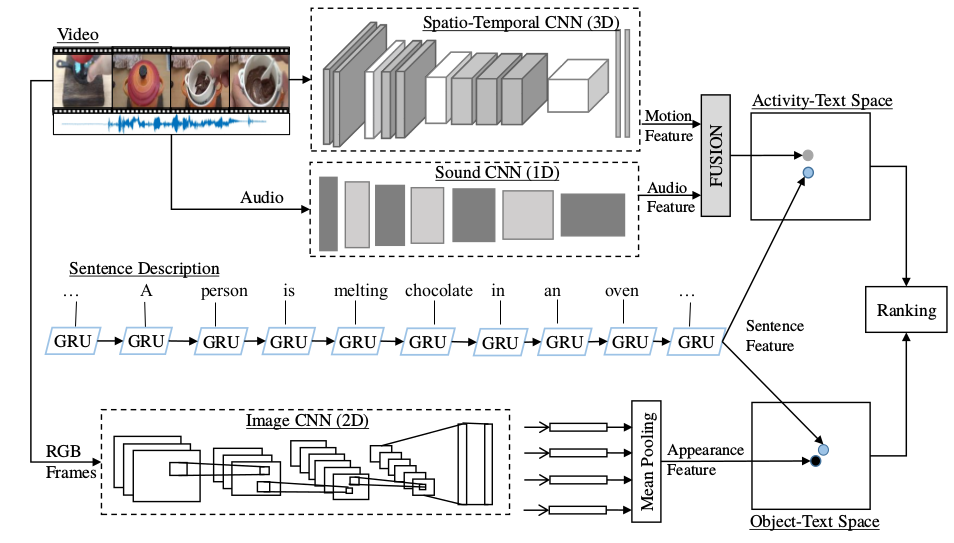
\includegraphics[width=\linewidth]{figures/related_mithun2018}
    \caption[Mithun等人~\cite{mithun2018learning}的活动-文本空间和物体-文本空间模型结构图]{\textbf{活动-文本空间和物体-文本空间模型结构图},来自~\cite{mithun2018learning}。}
    \label{fig:related_mithun2018}
\end{figure*}

而在视频片段检索领域,Yu等人~\cite{vsrel2020}使用了类似的做法,他们首先使用预训练的卷积神经网络VGG提取视频的帧图像特征,并使用平均池化的操作得到视频的物体特征,另外,他们还使用一个双流的卷积神经网络temporal segment network(TSN)~\cite{wang2016temporal}来提取视频的活动特征,该双流网络同时以帧图像和视频的光流作为输入。同样,他们单独地为这两类特征学习一个公共空间,并使用平均的方式后融合这两个公共空间。

考虑到视频具有非常复杂的信息,Miech等人在文献~\cite{miech2018learning}中提出的嵌入专家混合模型(Mixture of embedding experts,MEE) 使用多种视频的特征,包括ResNet-152对视频帧图像提取的物体特征,由I3D提取的视频的动作特征,由audio CNN提取视频的音频特征,他们还使用dlib框架~\footnote{\url{http://dlib.net/}}检测视频内的人脸并使用该框架里在人脸识别任务预训练的ResNet提取这些人脸特征,然后他们使用最大值池化对物体特征、动作特征和人脸特征在时间维度上进行池化,并使用NetVLAD对音频特征进行聚合,从而得到这视频级的这四种特征。而对于文本表示,他们先使用word2vec对句子的每个单词提取得到稠密特征,然后使用NetVLAD对单词特征进行聚合操作从而得到句子的特征表示。然后他们使用门控嵌入模块(Gated Embedding Module)来对这两种模态的特征进行处理,具体如公式~\ref{eq:gated-embedding-module}所示,
\begin{equation}
    \label{eq:gated-embedding-module}
    \begin{aligned}
        & Y_1 = W_1 X + b_1 \\
        & Y_2 = Y_1 \circ \sigma(W_2Y_1 + b_2) \\
        & Y = \frac{Y_2}{||Y_2||_2}
    \end{aligned}
\end{equation}
其中,$X$是输入的特征向量,$W_1$,$W_2$, $b_1$, $b_2$是可学习的参数,$\sigma$是sigmoid激活函数,$\circ$表示两个向量逐元素相乘。即对于每种视频特征,他们使用文本特征和该视频特征经过Gated Embedding Module处理,然后计算两种处理后的特征之间的余弦相似度,从而对于每对视频-文本对会产生四个余弦相似度,然后他们使用文本特征计算这四个相似度的权重,并根据该权重对这四个相似度加和得到视频-文本对的总相似度。他们的整体模型图如图~\ref{fig:related_miech2018}所示。

\begin{figure*}[tbh!]
    \centering
    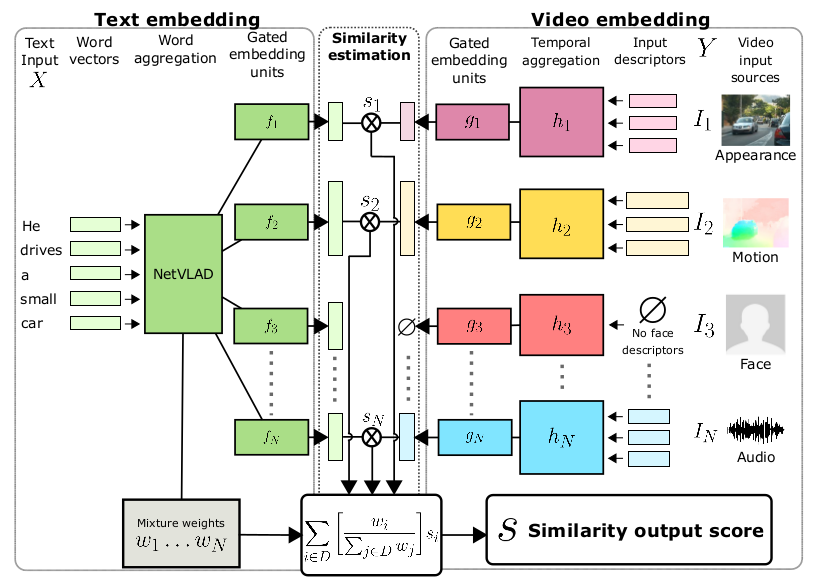
\includegraphics[width=\linewidth]{figures/related_miech2018}
    \caption[Miech等人~\cite{miech2018learning}的Mixture of embedding experts模型结构图]{\textbf{Mixture of embedding experts模型结构图},来自~\cite{miech2018learning}。}
    \label{fig:related_miech2018}
\end{figure*}

Liu等人~\cite{liu2019use}尽可能地挖掘了视频信息,他们提取了视频的物体特征、场景特征、动作特征、人脸特征、字符特征(optical character recognition,OCR)、言语(speech)特征和音频(audio)特征。他们首先使用深度卷积神经网络SENet-154~\cite{hu2019squeeze}模型提取视频帧图像的物体特征,在Places365~\cite{zhou2018places}数据上预训练的DenseNet-161~\cite{huang2017densely}提取帧图像的场景特征,双流卷积神经网络I3D提取连续帧图像的动作特征。而对于人脸特征,他们先使用人脸目标检测网络SSD~\cite{liu2016ssd}来提取帧图像中的人脸,然后再使用在VGGFace2~\cite{cao2018vggface2}数据上预训练的ResNet-50提取每个检测出的人脸的特征。对于OCR特征,他们先使用文本检测模型PixelLink~\cite{deng2018pixellink}来定位图像中的文本位置,然后每个文本框内的图像区域经过一个在文本识别数据Synth90K~\cite{liu2018synthetically}的模型~\cite{jakub-mm19}得到一序列字符串的文本,最后文本的每个单词的向量由预训练的word2vec模型提取。对于言语特征,他们使用谷歌云的API来对声音提取单词,然后得到的句子的单词的向量同样由word2vec模型提取。对于音频特征,他们使用在Youtube-8m~\cite{abuelhaija2016youtube}上预训练的audio CNN~\cite{hershey2017cnn}提取。最后,他们使用平均池化的方法来处理这些帧图像的物体特征、场景特征、动作特征和人脸特征,而使用NetVLAD的方法聚合OCR特征、言语特征和音频特征,从而最终得到视频级的相应的特征表示。为了融合所有的这些视频级特征,他们首先将这些特征做了线性投影,将所有特征转换到相同维度的特征,然后计算两两特征之间的关系,然后根据这个关系对转换后的特征进行缩放处理得到新的特征表示,使得有效的信息的权重加大,而冗余或者无效的信息被抑制,从而为模型提供了更加准确有效的特征作为输入。最终所有的视频特征都经过Gated Embedding Module~\cite{miech2018learning}处理,具体如公式~\ref{eq:gated-embedding-module},然后对所有的输出进行拼接并做L2规范化,得到最终的视频特征。而对于文本的表示,他们先用预训练的word2vec模型对句子的每个单词进行编码,然后这些单词编码再经过OpenAI-GPT~\cite{radford2018improving}模型,最后所有的输出通过NetVLAD进行聚合从而得到整个句子的编码,为了计算句子与视频的相似度,他们使用Gated Embedding Module为每个视频特征对句子编码进行处理,从而得到与视频特征维度相同的句子特征。他们使用余弦相似度计算句子与视频的相似度,并使用双向的排序损失函数(bidirectional marginal ranking loss)监督模型的训练。这种方法尽可能地使用了视频的信息,并且通过拼接的方法为每个视频特征学习跨模态计算的子空间,并将各个子空间的相似度相加融合。

Dong等人在文献~\cite{dong2018predicting}和Li等人在文献~\cite{li2019w2vv++}中通过拼接的方式融合了三种文本编码特征,即bag-of-words(bow)、word2vec和GRU,并且使用ResNet-152、ResNeXt-101为视频提取视觉特征。Dong等人~\cite{dong2018predicting}将拼接后的文本特征投影到视觉特征空间,在视觉特征空间中计算两种模态的距离。而Li等人~\cite{li2019w2vv++}将文本特征投影到视觉特征空间或将两种模态的特征同时投影到公共的隐空间,并在公共空间中计算文本和视频的余弦相似度。而Dong等人在文献~\cite{dong2019dual}进一步提出使用对偶的多层编码方式分别对文本和视频进行编码表示,他们的模型结构如图~\ref{fig:related_dong2019}所示,他们分别使用多层相似的编码方式对视频的帧特征和文本编码,即使用bow,bidirectional GRU(biGRU),并使用1D-CNN作用在bi-GRU的输出的所有隐藏层特征(biGRU-CNN),而在视频编码上,他们先使用ResNet-152对视频的帧图像提取视频特征,然后使用平均池化、biGRU和biGRU-CNN这三种方式对帧图像特征进行聚合得到三种层次的视频级特征,他们分别对文本的三种编码特征对视频的三种编码得到的视频特征进行拼接来表示文本和视频,最后使用全连接层对这两种模态的特征投影到公共的隐空间,从而在这个学习的隐空间中可以计算文本和视频的余弦相似度。

\begin{figure*}[tbh!]
    \centering
    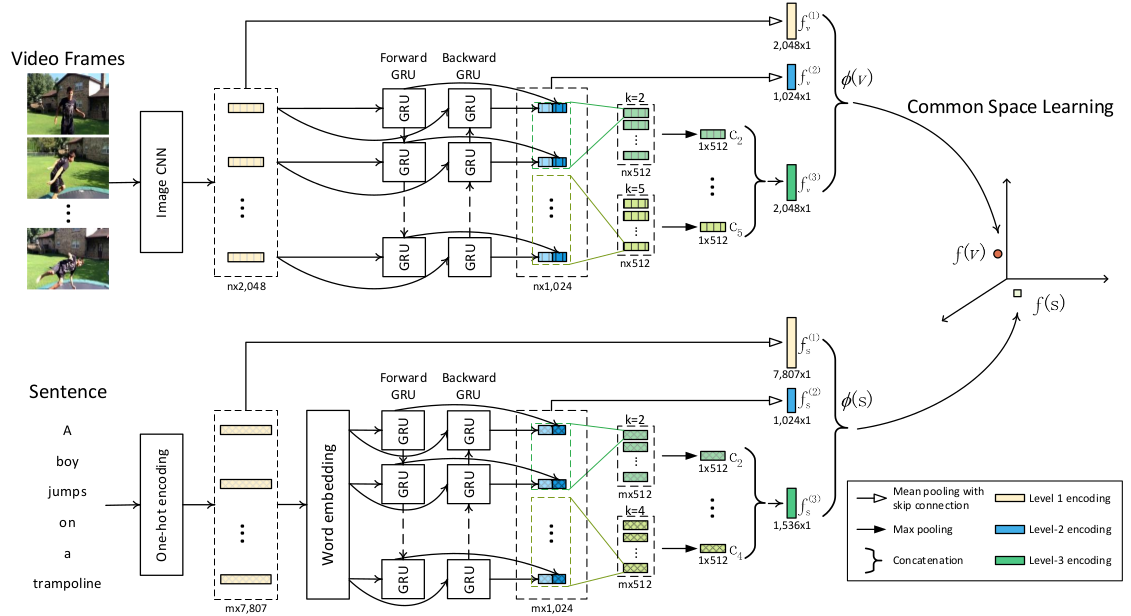
\includegraphics[width=\linewidth]{figures/related_dong2019}
    \caption[Dong等人~\cite{dong2019dual}的对偶编码网络模型结构图]{\textbf{对偶编码网络模型结构图},来自~\cite{dong2019dual}。}
    \label{fig:related_dong2019}
\end{figure*}

\section{本章小结}
本章首先回顾了近四年的TRECVID评测中的即席检索视频系统,可以发现即席视频检索技术是逐渐由基于概念的模型向基于完全深度学习的模型发展,近年来越来越多的即席视频检索技术是基于完全深度学习的方法,并取得了优秀的成绩。本文另一方面也回顾了一些基于文本的跨模态视频检索技术,因为文本与视频都是具有非常复杂语义信息的媒体数据,这些技术都采用了多种视频特征或者文本特征,并在同一个模型下融合这些特征,得到了更加出色检索的效果。
